\documentclass[a4paper]{article}

\usepackage[utf8]{inputenc}
\usepackage[english]{babel}
\usepackage{hyperref}
\usepackage{graphicx}
\usepackage{amsmath,amssymb,amsthm}
\usepackage{siunitx}
\usepackage{xcolor}
\usepackage{multicol}
\usepackage{caption}
\usepackage{appendix}
\usepackage{pdfpages}
\usepackage{fixltx2e}
\usepackage[version=4]{mhchem}
\usepackage{url}
\usepackage{subcaption}
\usepackage{subfig}
\usepackage[justification=centering]{caption}
\usepackage[thinc]{esdiff}
\usepackage[bottom]{footmisc}


\date{\today}
\author{Thomas Brzeski \and  Victor Dejans}
\title{Kinematic and Dynamic Analysis of a Linkage\\ Walschaerts Valve Gear}


\begin{document}

\maketitle

\section*{Introduction}

In the context of the subject \textit{Beweging en trillingen (H01N0A)} this report treats the analysis of the linkage in a Walschaerts valve gear, a system that is used in steam locomotives. The linkage that is studied in this report is based on that in figure~\ref{fig:basistekening}.

In a first section we define all links and joints with their geometric properties in the way we used them for the assignment. We also make the motion analysis of the linkage.

Second is the kinematic analysis which finds the positions, velocities and accelerations of each bar.

The final section reports upon the inverse dynamic analysis which finds the forces and torques on the linkages' joints when a driving torque is applied to the train's wheel.



\tableofcontents
\clearpage

\section{Definition of the mechanism}

Walschaerts valve gear is a linkage that was used in steam locomotives. It connects the steam pistons and the train's wheels in a way that also regulates the steam flow.

Although in real life the pistons are the driving bodies and the wheels is the driven bodies, the assistants recommended us to analyse the mechanism in the opposite way. In this assignment, the driving torque is thus applied to the wheel instead of the pistons.

\begin{figure}[h]
	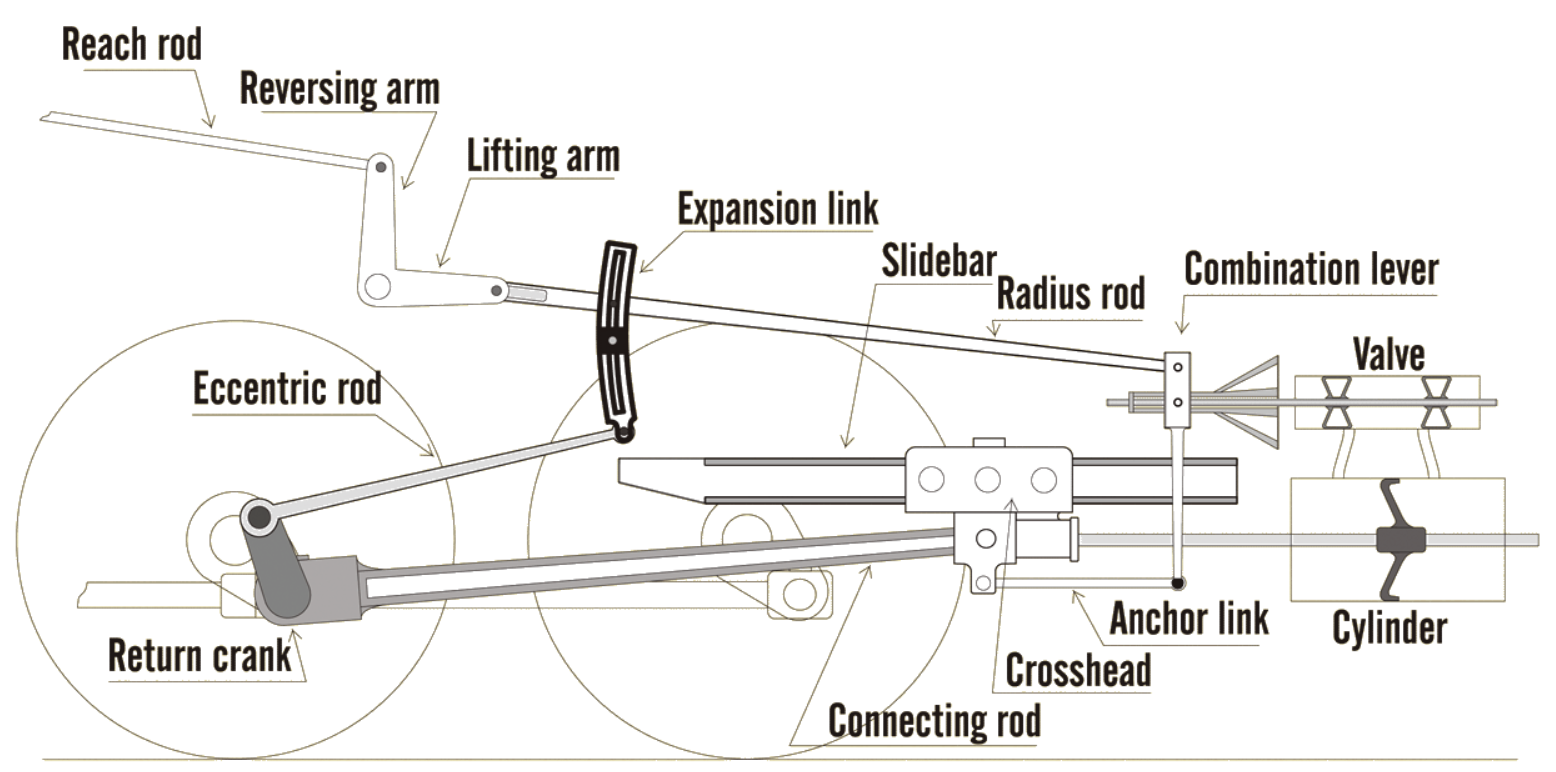
\includegraphics[width=0.9\textwidth]{wvgverslag.png}
	\centering
	\caption{Example of a Walschaerts valve gear. \cite{ove06}}
	\label{fig:basistekening}
\end{figure}

\subsection{Schematic of the mechanism and definition of the parameters}

As shown in figure~\ref{fig:schematic}, the linkage has twelve bodies.

\begin{itemize}
	\item Body \textbf{(1)} is the train. This is the ground to which other bodies are fixed.
	\item Body \textbf{(2)} is the wheel of the train. Its rotation point (A) is fixed in the origin of the xy-plane. The ends of bars (3) and (12) are eccentrically attached to the wheel with hinges (B) and (C) respectively.
	\item Bodies \textbf{(3)}, \textbf{(4)}, \textbf{(7)}, \textbf{(8)}, \textbf{(10)} and \textbf{(12)} are straight bars.
	\item Body \textbf{(5)} is massless and is used to make a special joint between bar (4) and bar (7). It is attached to bar (4) with a prismatic joint (I) and to bar (7) with a hinge (H).
	\item Bar \textbf{(6)} is a kinked, L-shaped bar which consists of two parts of 95~\si{cm} long that are fixed to each other in an angle of 90~\si{degrees}. The two ends of this L-shaped bar are fixed to the ground (1) and to bar (7) with hinges.
	\item Bodies \textbf{(9)} and \textbf{(11)} are the pistons of the valve gear. Both pistons are fixed to the ground (1) with prismatic joints ((L) and (P) respectively) that only allow movement in the x-direction. Their dimensions are shown in figure~\ref{fig:pistons}.
\end{itemize}

The dimensions of the bars and other bodies are defined in tables~\ref{tab:lengths} and~\ref{tab:angles}.

All bodies in this linkage are made of steel which has a density \(\rho_{steel} = 7800~\si{kg/m^3}\) \cite{steel1}.

\begin{figure}
	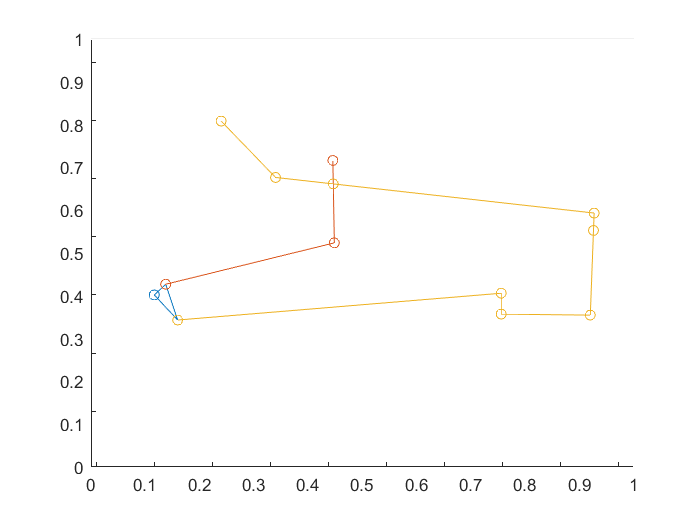
\includegraphics[width=\textwidth]{schematic.png}
	\centering
	\caption{Schematic representation of the studied linkage. The numbers indicate the 12 bodies. The letters indicate the 16 joints.}
	\label{fig:schematic}
\end{figure}

\begin{table}
	\centering
	\begin{tabular}{lr}
		\hline
		Bar & Length \((\si{cm})\) \\
		\hline
		1 between A and E & 321 \\
		1 between A and F & 385 \\
		2 between A and C & 27 \\
		2 between A and B & 59 \\
		3 between C and D & 299 \\
		4 between D and F & 142 \\
		6 between E and G (in a straight line) & 135 \\
		7 between G and H & 100 \\
		7 between H and J & 452 \\
		8 between J and K & 30 \\
		8 between K and M & 146 \\
		10 between O and M & 158 \\
		12 between B and N & 559 \\
		Y-coordinate of joint K \footnotemark & \\
		Y-coordinate of joint N \footnotemark & \\
		\hline
	\end{tabular}
	\footnotetext{Because}
	\caption{Lenghts of the bars and the wheel. Bars' numbers and joints' letters as indicated in figure~\ref{fig:schematic}.}
	\label{tab:lengths}
\end{table}

\begin{table} 
	\centering
	\begin{tabular}{lr}
		\hline
		Line segment & Angle to the positive x axis \((\si{degrees})\) \\
		\hline
		[AE] & 69 \\
		\text{[AF]} & 37,0188 \\
		\hline
	\end{tabular}
	\caption{Unvariable angles in the linkage's ground. Joints' letters as indicated in figure~\ref{fig:schematic}. Variable angles are calculated in section \ref{sec:kin}}
	\label{tab:angles}
\end{table}


\begin{figure}
	\centering
	
	\begin{subfigure}[b]{.4\textwidth}
		\centering
		\label{fig:piston9}
		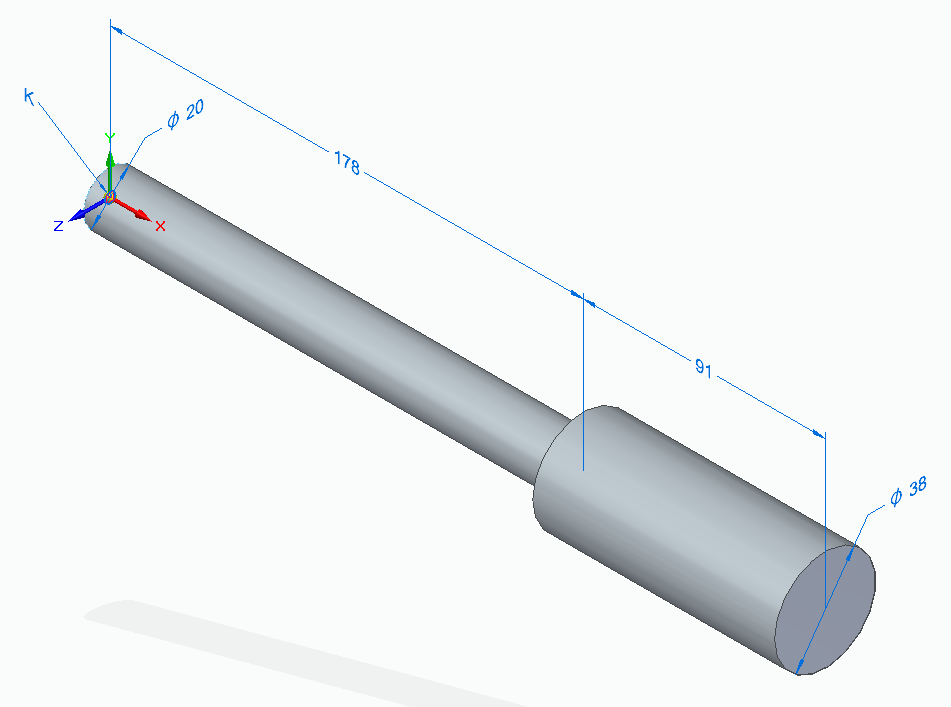
\includegraphics[width=\textwidth]{piston9.png}
		\caption{Piston (9).\centering}
	\end{subfigure}
	\hfill
	\begin{subfigure}[b]{.4\textwidth}
		\centering
		\label{fig:piston11}
		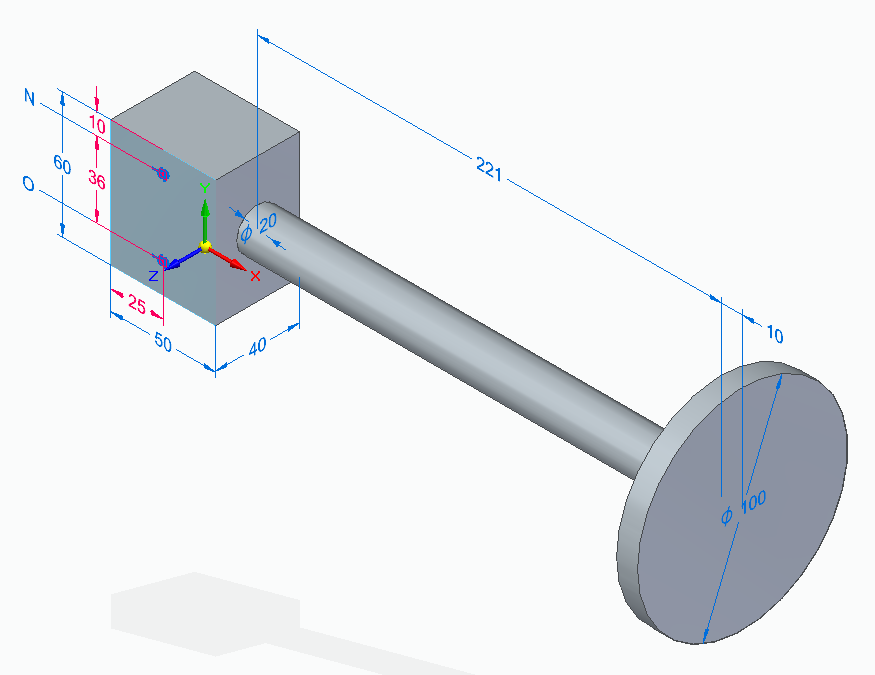
\includegraphics[width=\textwidth]{piston11.png}
		\caption{Piston (11).\centering}
	\end{subfigure}

	\caption{Pistons (9) and (11) with their dimensions in cm and with their joints with other bodies.}
	\label{fig:pistons}
	
\end{figure}



\subsection{Motion analysis}

The Walschaerts valve gear is a twelve bar linkage system with sixteen joints. This makes the mobility \(M=3*(12-1)-16*2=1\). This means the system has one degree of freedom.


\newpage

\section{Kinematic analysis}
\label{sec:kin}

In the kinematic analysis we apply a driving torque to the train's wheel (body (2)) and see how the other bars react. 

The driving torque is applied to body (2) in point (A) and makes it turn with a constant angular velocity as defined in equation~\ref{eq:dphi2}, where \(\phi_2(t)\) is the angle that section [AB] of the wheel makes with the positive x axis.

\begin{equation}
	\phi_2(t) = \pi*t~rad \\
	\label{eq:phi2}
\end{equation}
\begin{equation}
	\diff{\phi_2(t)}{t} = \pi~rad/s \\
	\label{eq:dphi2}
\end{equation}
\begin{equation}
	\diff[2]{\phi_2(t)}{t} = 0~rad/s^2\\
\end{equation}

The kinematic analysis looks for the positions, velocities and accelerations of the other bodies in the linkage. The ten unknowns are \(\phi_3(t)\), \(\phi_4(t)\), \(r_{4a}(t)\) (the length of the part of bar (4) between joint (D) and joint (I)), \(\phi_6(t)\), \(\phi_7(t)\), \(\phi_8(t)\), \(x_9(t)\) (the x coordinate of joint (K)), \(\phi_{10}(t)\), \(x_{11}(t)\) (the x coordinate of joint (N)) and \(\phi_{12}(t)\) and their first and second order derivatives. The angles are defined in figure~\ref{fig:schematic}.

The analysis is done for 201 time samples of 0,05~s each.

\subsection{Position analysis}

In order to find the ten unknown positions, a set of ten "loop closure equations" is solved for each time step. A loop closure equation is the sum of all x or y vector components of linkage bodies that form a closed loop. These sums are all equal to zero. This results in a set of ten equations which are listed below in vector form \footnote{These five vector equations define the ten equations because each vector can be split in one x component and one y component.}.


\begin{subequations}
\begin{equation}
	\vec{AB}+\vec{CD}+\vec{DF}-\vec{AF}=0
\end{equation}

\begin{equation}
	-\vec{GE}+\vec{GJ}-\vec{MJ}-\vec{OM}-\vec{NO}-\vec{BN}-\vec{AB}+\vec{AE}=0
\end{equation}

\begin{equation}
	\vec{AC}+\vec{CD}+\vec{DI}-\vec{GH}+\vec{GE}-\vec{AE}=0
\end{equation}

\begin{equation}
	\vec{AC}+\vec{CD}+\vec{DI}+\vec{HJ}-\vec{KJ}-\vec{AK}=0
\end{equation}

\begin{equation}
	\vec{AB}+\vec{BN}-\vec{AN}=0
\end{equation}

\label{eq:loopclosurevec}
\end{subequations}

%	\begin{subequations}
%		\begin{equation}
%		r2c*cos(\phi_2+\phi_A)+r3*cos(\phi_3)+r4*cos(\phi_4)-r1b*cos(\phi_AF)=0
%	\end{equation}
%	
%	\begin{equation}
%	r2c*sin(\phi_2+\phi_A)+r3*sin(\phi_3)+r4*sin(\phi_4)-r1b*sin(\phi_AF)=0
%	\end{equation}
%	\begin{equation}
%	%van knoop E naar knoop A langs driehoek8 en terug
%		-r6*cos(\phi_6)+r7*cos(\phi_7)-r8*cos(\phi_8)-r10*cos(\phi_10)-r11*cos(\phi_11)-r12*cos(\phi_12)-r2b*cos(\phi_2)+r1a*cos(\phi_AE)=0
%	\end{equation}
%	\begin{equation}
%	-r6*sin(\phi_6)+r7*sin(\phi_7)-r8*sin(\phi_8)-r10*sin(\phi_10)-r11*cos(\phi_11)-r12*sin(\phi_12)-r2b*sin(\phi_2)+r1a*sin(\phi_AE)=0
%	\end{equation}
%	\begin{equation}
%	%van knoop A naar knoop E langs bar3 en terug
%		r2c*cos(\phi_2+\phi_A)+r3*cos(\phi_3)+r4a*cos(\phi_4)-r7a*cos(\phi_7)+r6*cos(\phi_6)-r1a*cos(\phi_AE)=0
%	\end{equation}
%	\begin{equation}	r2c*sin(\phi_2+\phi_A)+r3*sin(\phi_3)+r4a*sin(\phi_4)-r7a*sin(\phi_7)+r6*sin(\phi_6)-r1a*sin(\phi_AE)=0
%	\end{equation}
%	\begin{equation}
%	%van knoop A naar prisma 9 en terug
%		r2c*cos(\phi_2+\phi_A)+r3*cos(\phi_3)+r4a*cos(\phi_4)+r7b*cos(\phi_7)-r8a*cos(\phi_8)-x9=0
%	\end{equation}
%	\begin{equation}
%	r2c*sin(\phi_2+\phi_A)+r3*sin(\phi_3)+r4a*sin(\phi_4)+r7b*sin(\phi_7)-r8a*sin(\phi_8)-y9=0
%	\end{equation}
%	\begin{equation}
%	%van knoop A naar prisma 11 langs bar12 en terug
%		r2b*cos(\phi_2)+r12*cos(\phi_12)-x11=0
%	\end{equation}
%	\begin{equation}
%	r2b*sin(\phi_2)+r12*sin(\phi_12)-y11=0
%	\end{equation}
%	\end{subequations}

The MATLAB function \texttt{loop\char`_closure\char`_eqs.m} lists all loop closure equations. In this case, we get a nonlinear system of equations because of the multiplication of the unknown variables \(\phi_4(t)\) and \(r_{4a}(t)\). The MATLAB function \texttt{fsolve} is used to solve this nonlinear set.

After solving this system for each of the 201 time samples, the MATLAB code returns values for each of the ten unknowns in function of the time. The plots of these ten variables are shown in figure~\ref{fig:kinpos}.

\begin{figure}
	\centering
	
	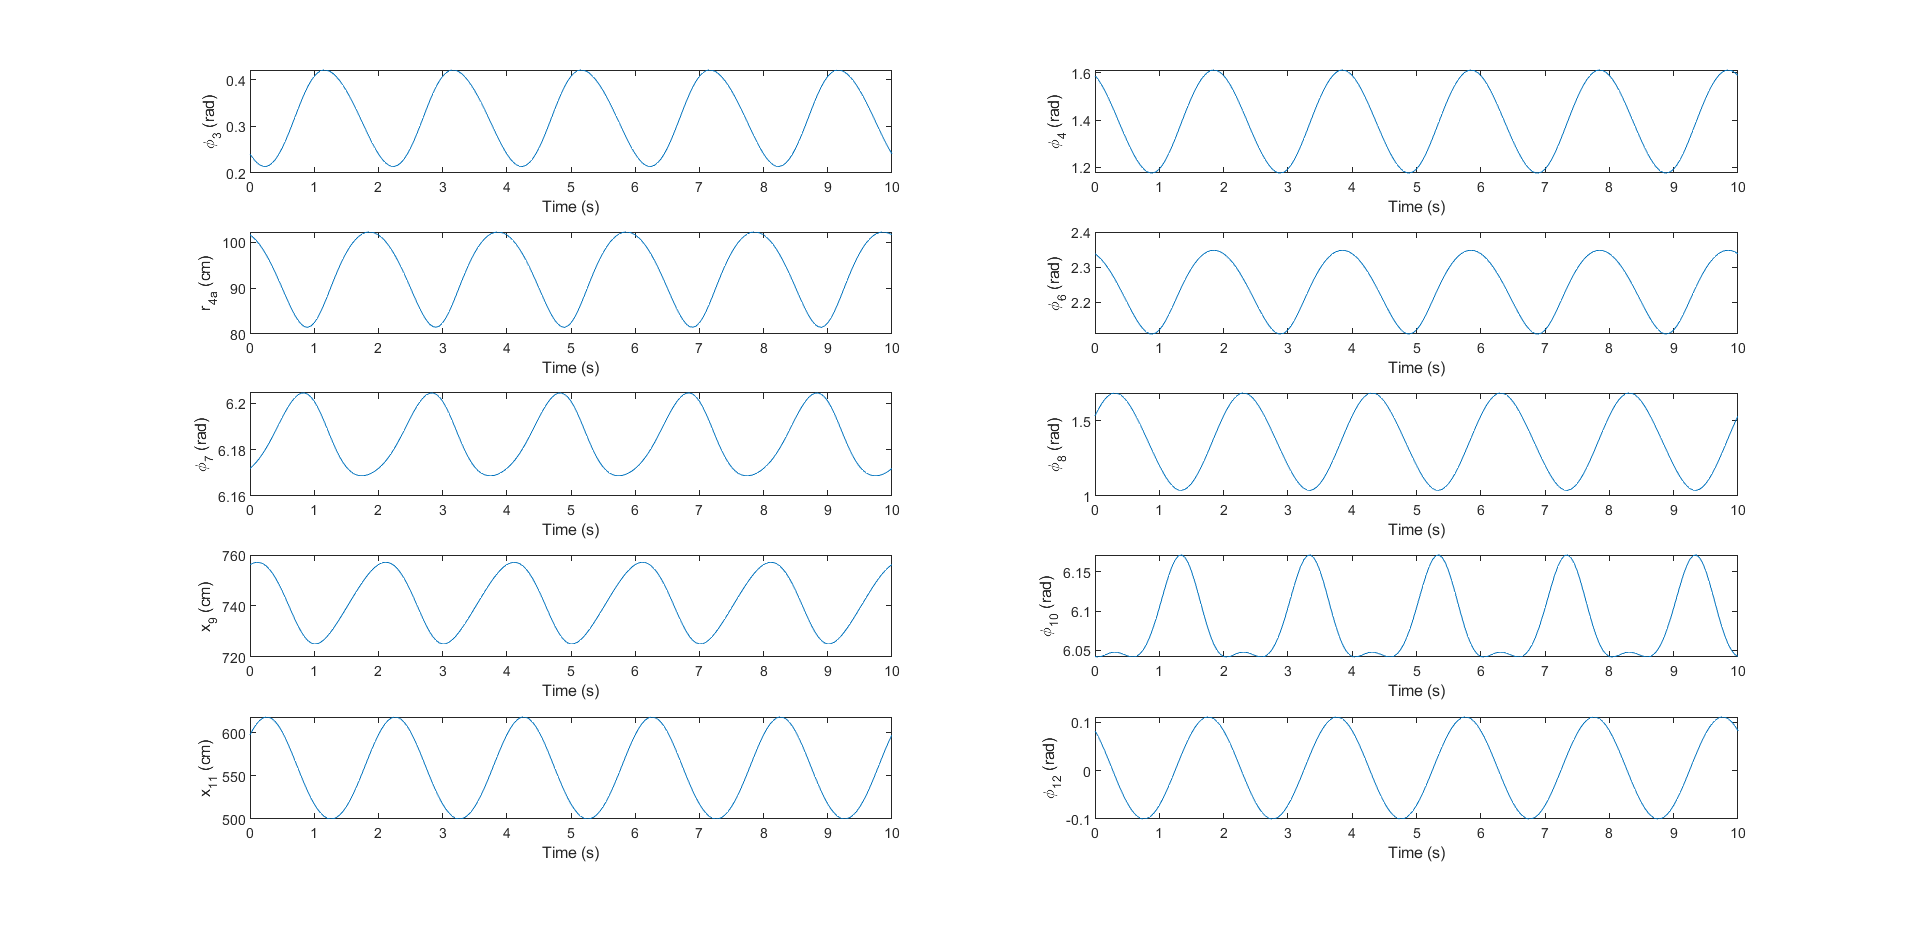
\includegraphics[width = \textwidth]{kinpos.png}
	
	\caption{Angles of the bodies (to the positive x axis), distance from joint (D) to (H) and x coordinates of the pistons (according to (A)) in function of time.}
	\label{fig:kinpos}
	
\end{figure}



\subsection{Velocity analysis}

The velocity analysis finds the ten unknown variables \(\diff{\phi_3(t)}{t}\), \(\diff{\phi_4(t)}{t}\), \(\diff{r_{4a}(t)}{t}\), \(\diff{\phi_6(t)}{t}\), \(\diff{\phi_7(t)}{t}\), \(\diff{\phi_8(t)}{t}\), \(\diff{x_9(t)}{t}\), \(\diff{\phi_{10}(t)}{t}\), \(\diff{x_{11}(t)}{t}\) and \(\diff{\phi_{12}(t)}{t}\).

The first order time derivatives of the loop closure equations~\ref{eq:loopclosurevec} are now used to find the unknown velocities. They are listed in the MATLAB function \texttt{velocity\char`_eqs}. The first order derivative of body (2) is known and is defined in equation~\ref{eq:dphi2}. 

The new set of loop closure equations is now linear because the derivative of the multiplication of \(\phi_4(t)\) and \(r_{4a}(t)\) contains no multiplication of the now unknown \(\diff{\phi_4(t)}{t}\) and \(\diff{r_{4a}(t)}{t}\).

The MATLAB code solves this system and returns values for the velocities of the bodies in function of the time. They are plotted in figure~\ref{fig:kinvel}.

\begin{figure}[h]
	\centering
	
	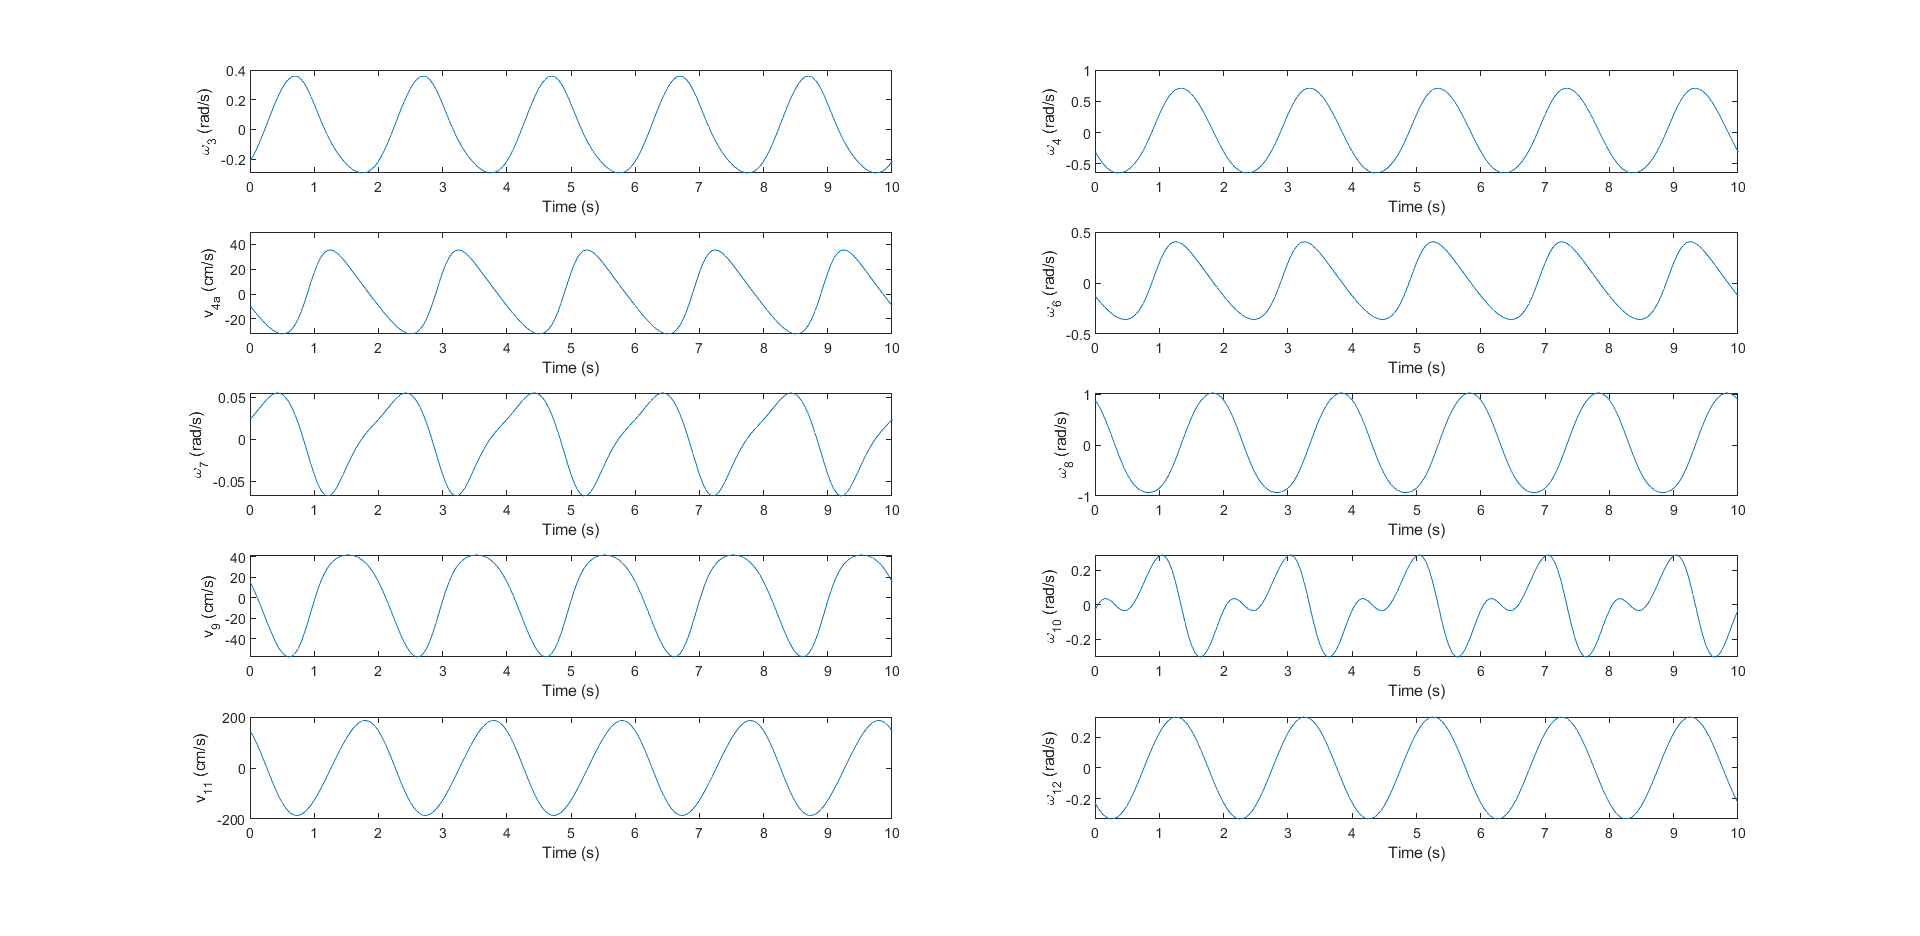
\includegraphics[width = \textwidth]{kinvel.png}
	
	\caption{Angular velocities of the bodies (to the positive x axis) and linear velocities of joint (H) (according to (D)) and of the pistons (according to (A)) in function of time.}
	\label{fig:kinvel}
	
\end{figure}

\subsection{Acceleration analysis}

The acceleration analysis finds the ten unknown variables \(\diff[2]{\phi_3(t)}{t}\), \(\diff[2]{\phi_4(t)}{t}\), \(\diff[2]{r_{4a}(t)}{t}\), \(\diff[2]{\phi_6(t)}{t}\), \(\diff[2]{\phi_7(t)}{t}\), \(\diff[2]{\phi_8(t)}{t}\), \(\diff[2]{x_9(t)}{t}\), \(\diff[2]{\phi_{10}(t)}{t}\), \(\diff[2]{x_{11}(t)}{t}\) and \(\diff[2]{\phi_{12}(t)}{t}\).

This happens analogously to the velocity analysis. The MATLAB code now solves a linear set of the second order time derivatives of the ten loop closure equations. These are listed in the MATLAB function \texttt{acceleration\char`_eqs}. The plots of the accelerations of the bodies are in figure~\ref{fig:kinacc}.

\begin{figure}
	\centering
	
	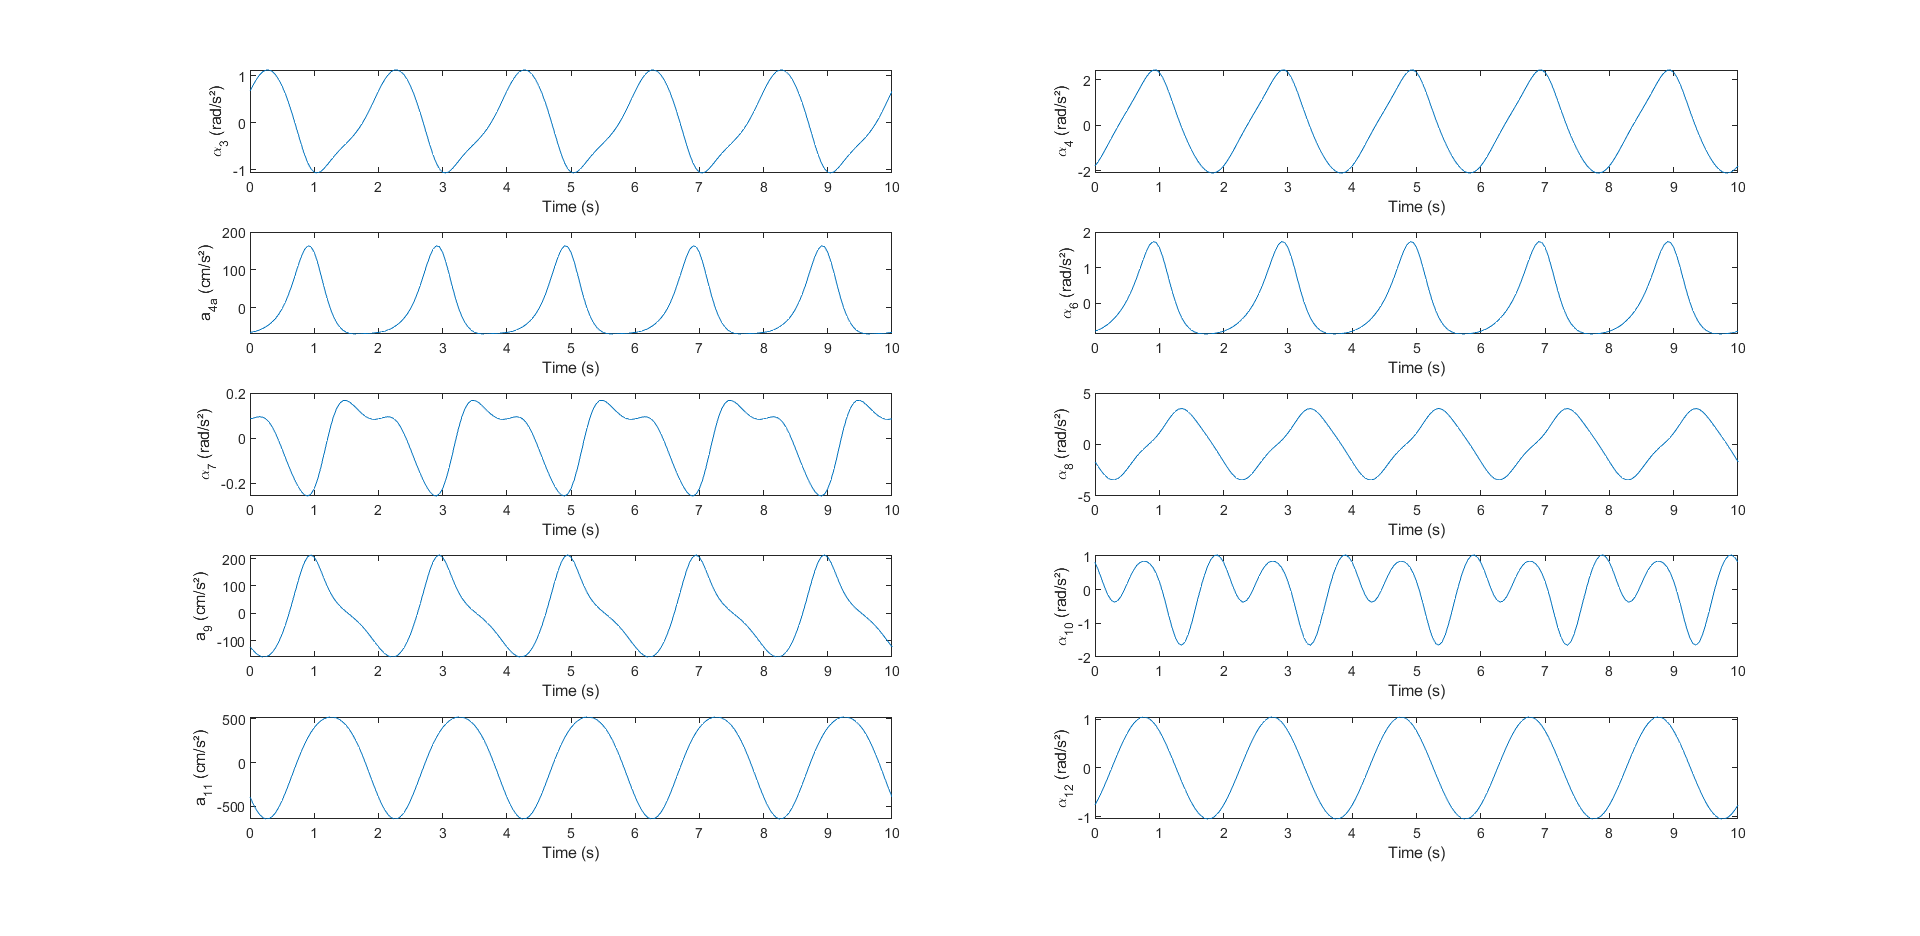
\includegraphics[width = \textwidth]{kinacc.png}
	
	\caption{Angular accelerations of the bodies (to the positive x axis) and linear accelerations of joint (H) (according to (D)) and of the pistons (according to (A)) in function of time.}
	\label{fig:kinacc}
	
\end{figure}

\subsection{Checking the results}

\section{Dynamic analysis}

\subsection{Inverse dynamic analysis without gravity}

\subsection{Inverse dynamic analysis with gravity}

\subsection{Checking the results}

\bibliographystyle{plain}
\bibliography{walschaerts}


\end{document}